
\chapter{Mbona Hatchery}

\section{Infrastructure.}

At the Mbona Hatchery we make use of Baths, Tanks and Ponds for the production of fry, fingerlings and table fish, see ~\ref{fig:HatcheriesLayout} for the layout of the Mbona Hatcheries operation.

\begin{figure}[H]
  \centering
   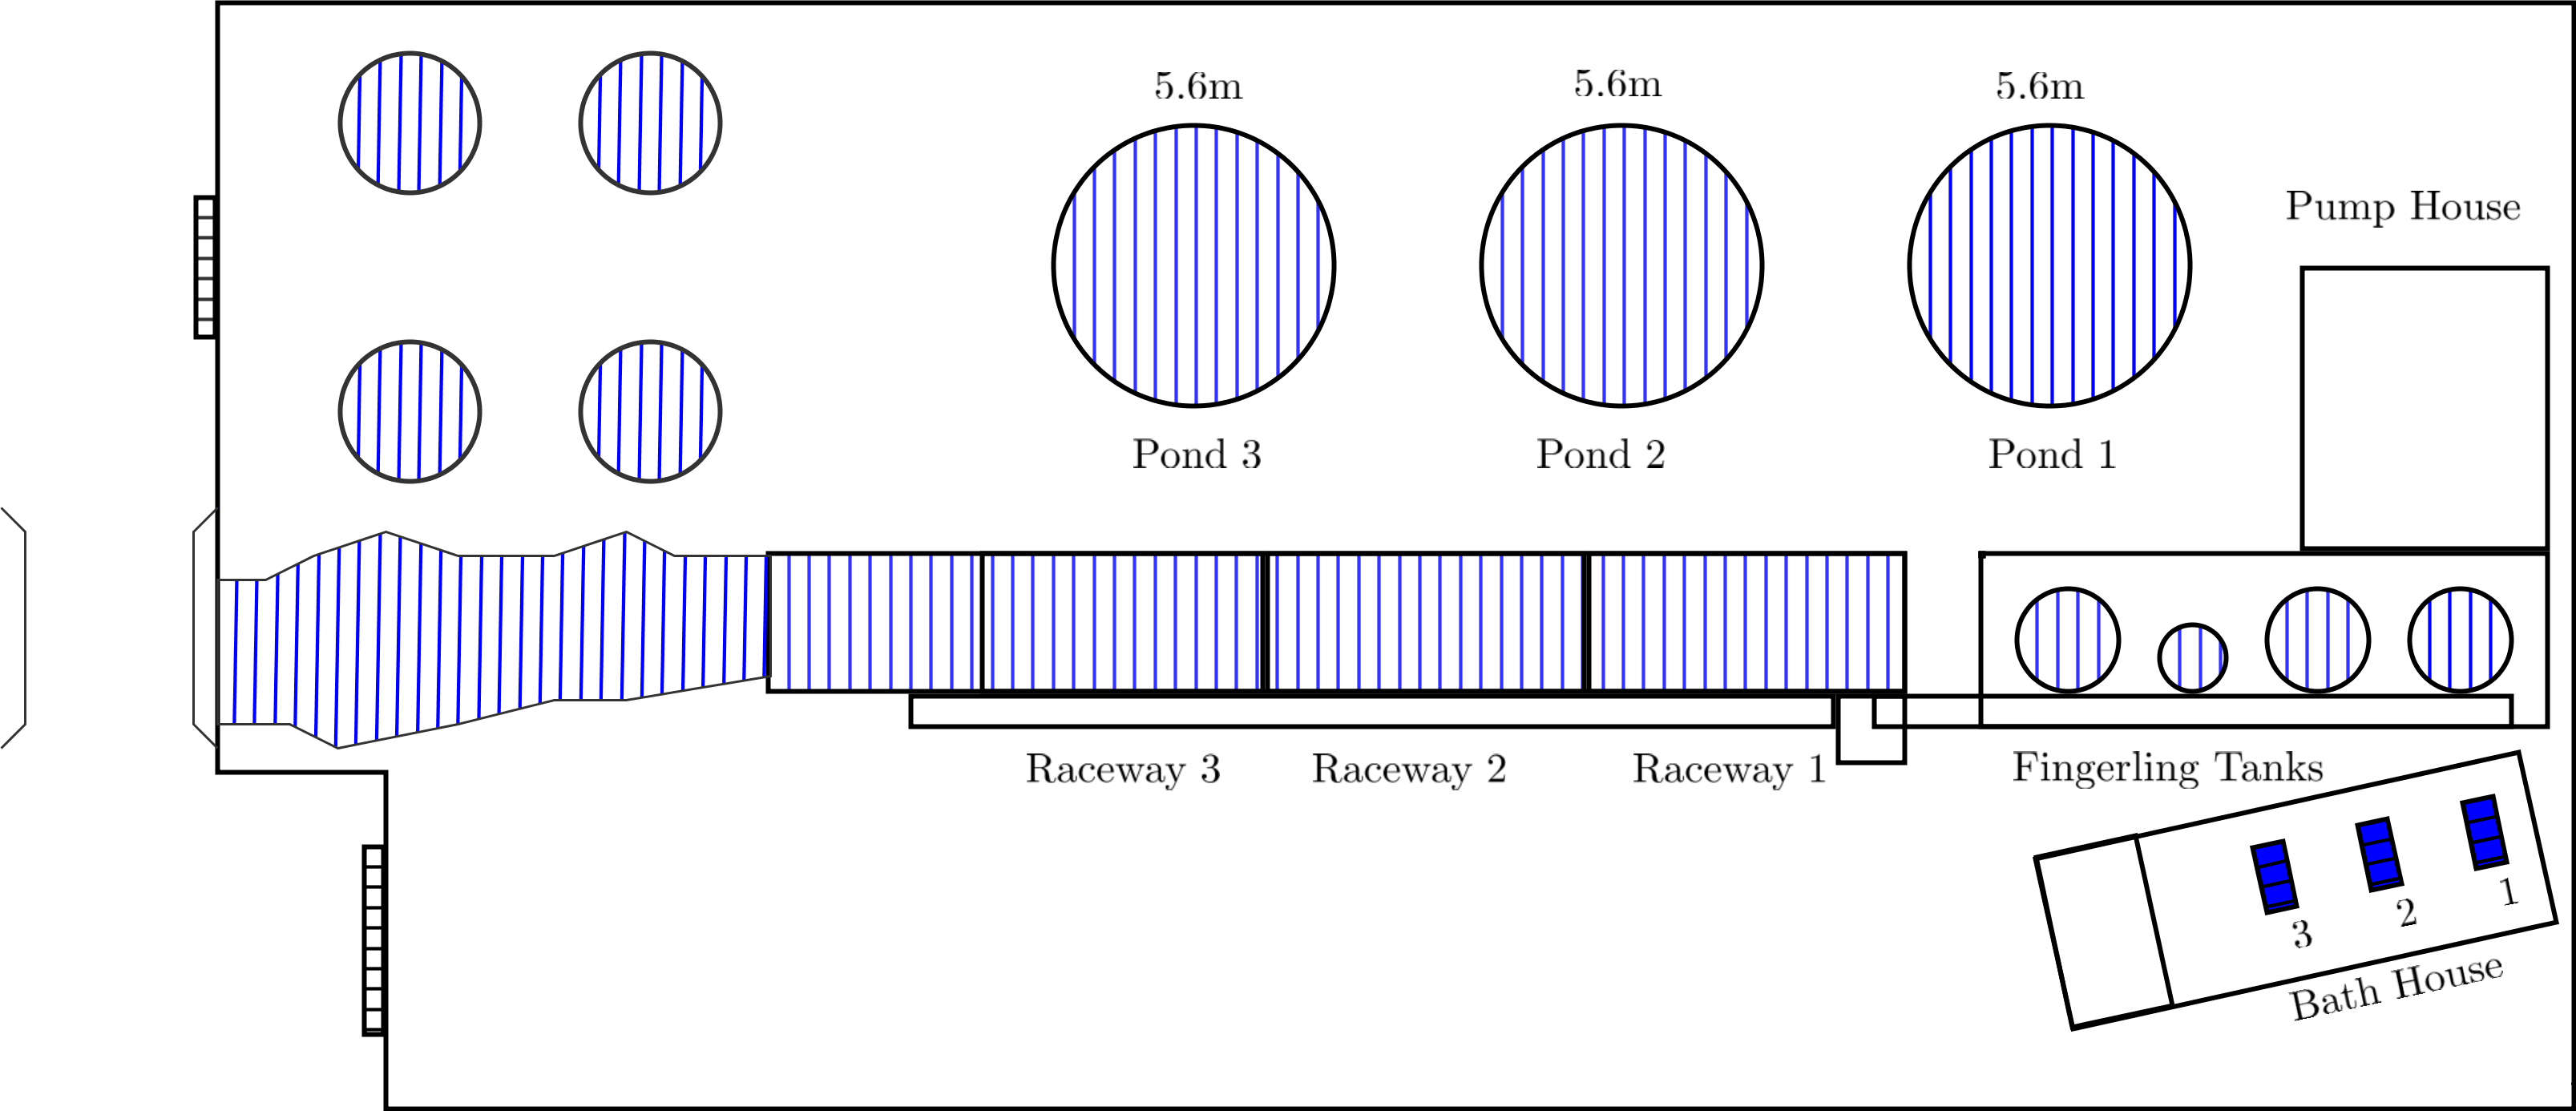
\includegraphics[scale = 0.15,angle=0,origin=c]{images/HatcheriesLayout.png}
  \caption{Mbona Hatcheries Layout.}
   \label{fig:HatcheriesLayout}
\end{figure}

\subsection{Hatching Baths} 

At the Mbona Hatchery we use a California hatching tray which is a screened, flat-bottomed tray that fits horizontally inside the rearing bath and is arranged so that water is forced through the eggs from below.

The tray is a container for incubation of eggs and sac fry. The bottom of the tray is a sieve material, on which the eggs and sac fry rest. They are placed in a Hatching Bath and they receive freshwater through the sieve from under the tray, as illustrated in figure~\ref{fig:HatcheryBaths}. 

\begin{figure}[H]
  \centering
   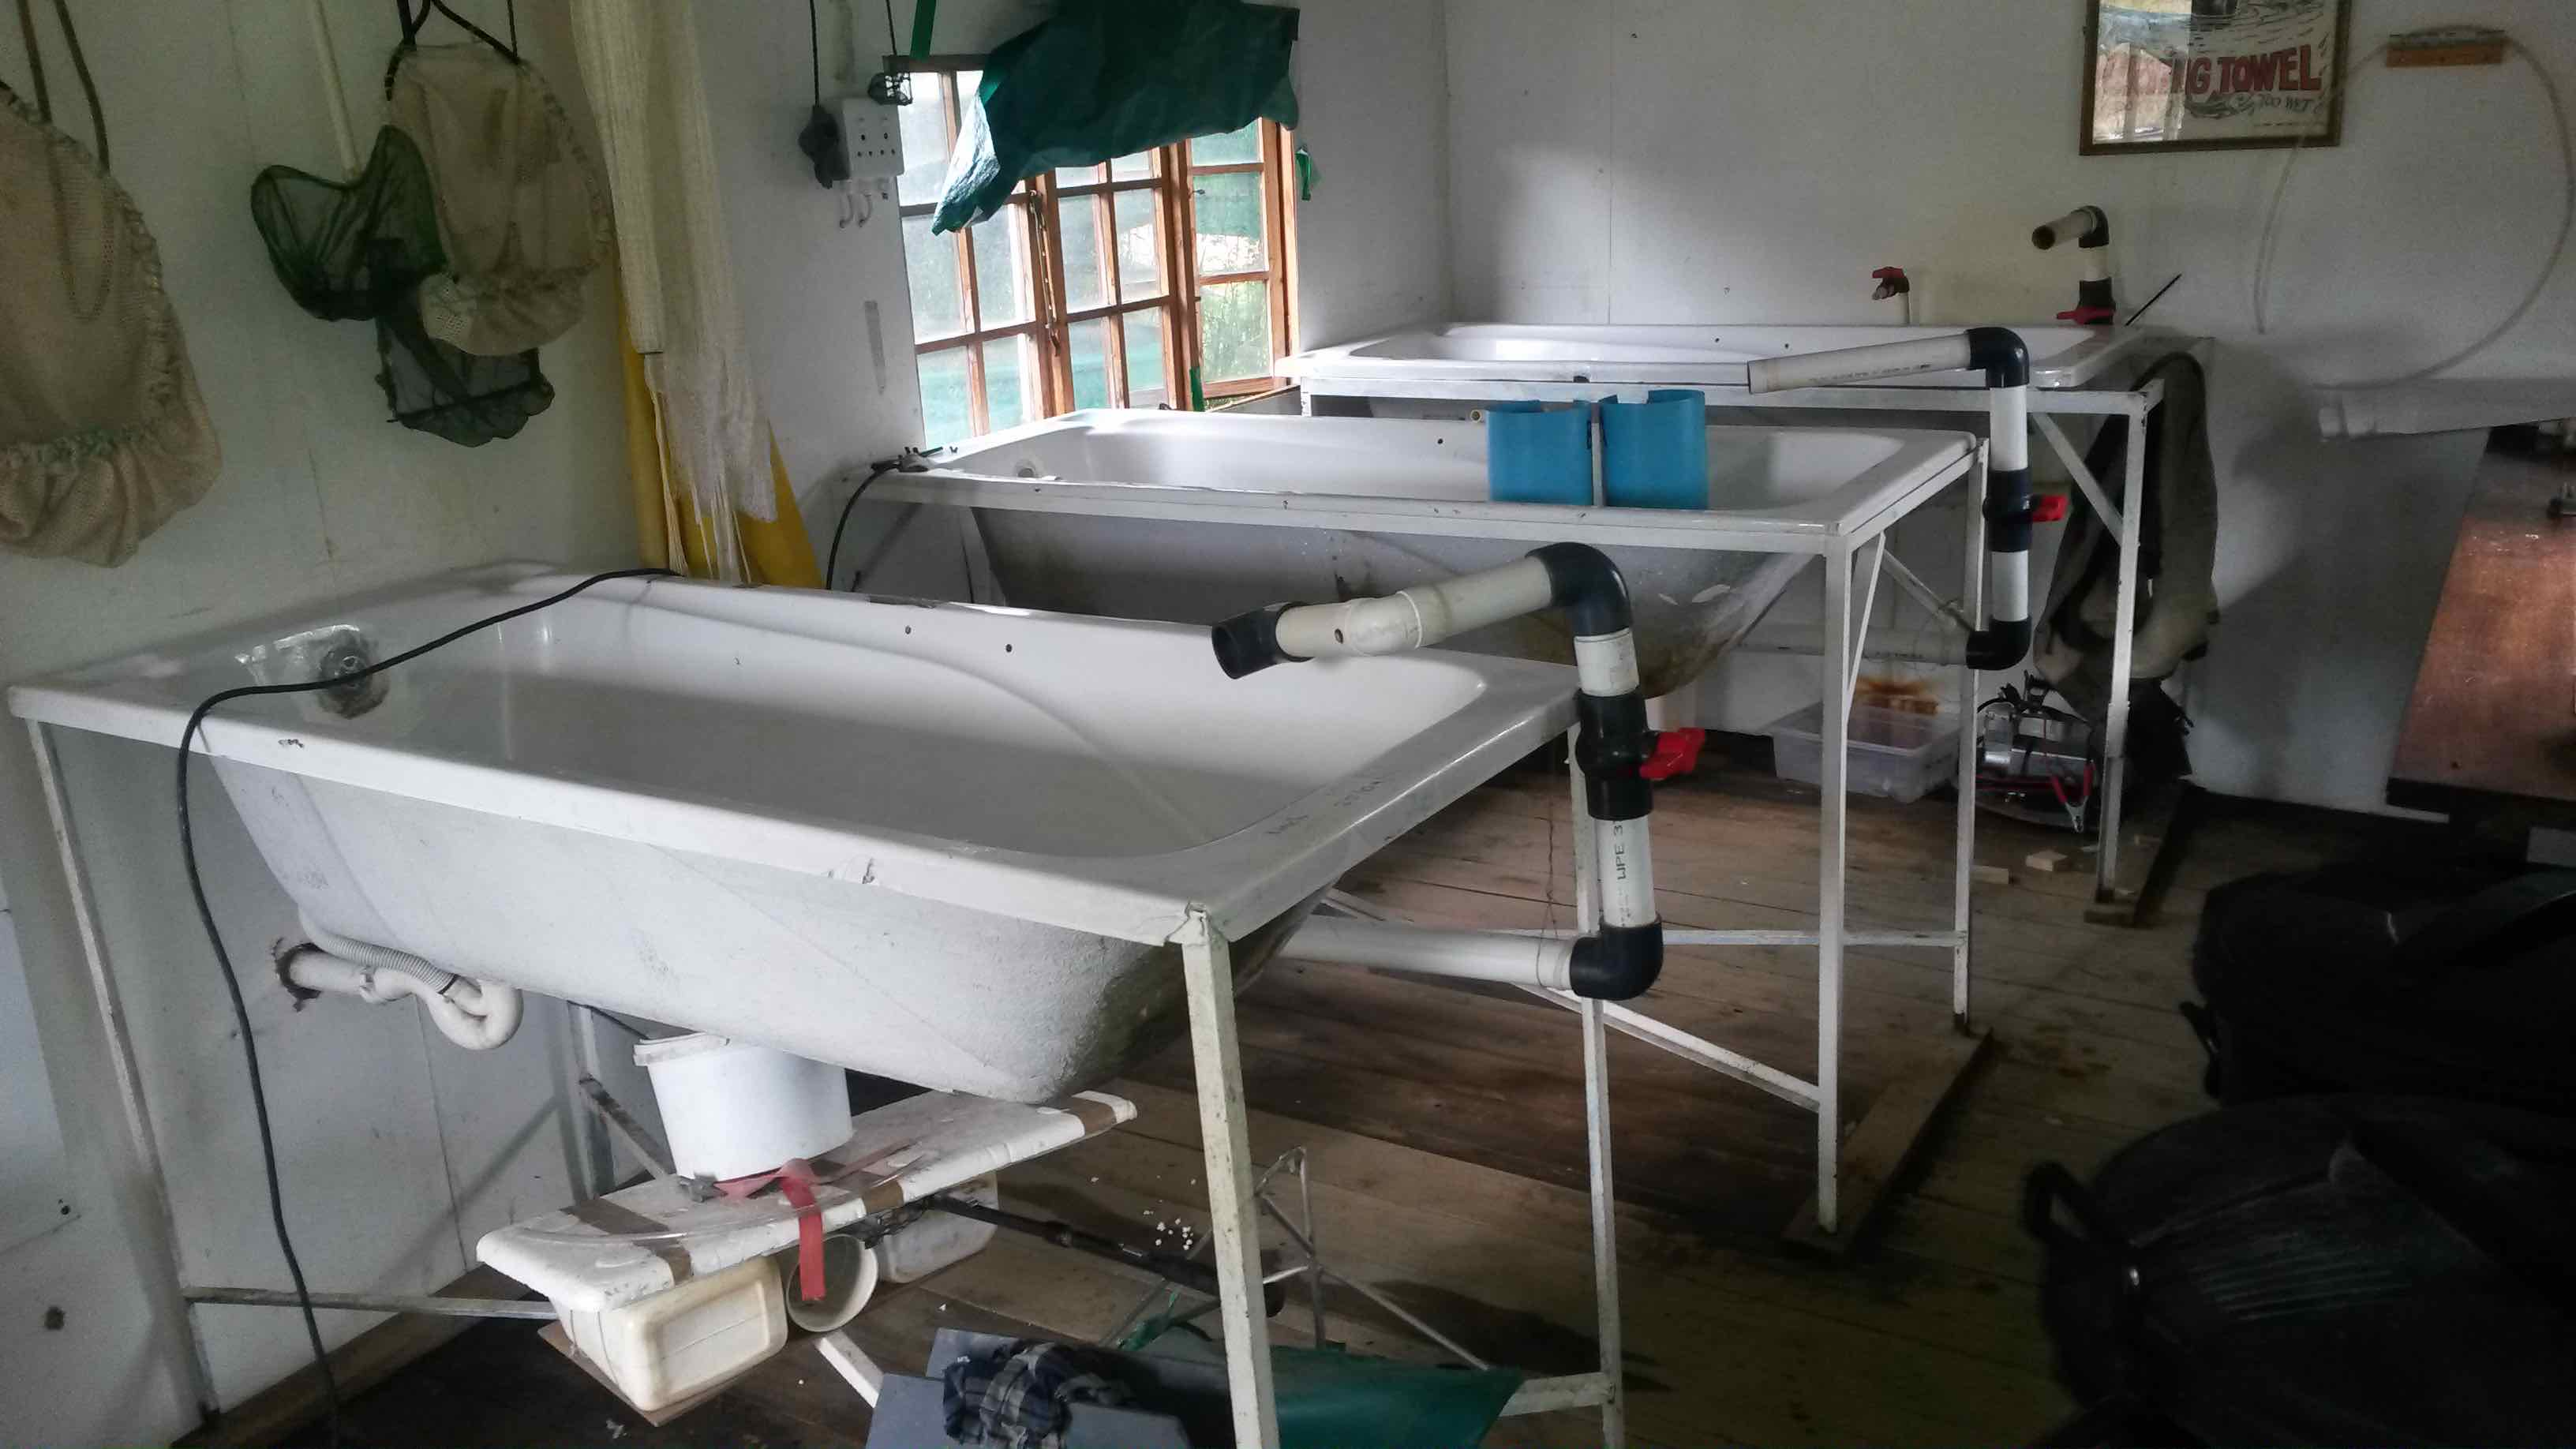
\includegraphics[scale = 0.1]{images/HatcheryBaths.jpg}
  \caption{Mbona incubator baths have one California type tray (size: 0.5 m � 0.4 m = 0.2 m2). When hatching trays are removed, the bath is used for rearing the fry.}
   \label{fig:HatcheryBaths}
\end{figure}


Although the material, shape and size of hatching trays may vary, the quantities of eggs and sac fry that can be incubated on them are similar. A hatching tray about 0.2 meter squared is needed for the incubation and hatching of 10 000 rainbow trout eggs. Later, the required space increases, because 10 000 swim-up fry need 5 times more space (about 1 meter squared) with about 0.5 m depth. The required quantity of water in these devices should be ensured and adjusted as presented in the graphs of the previous chapter.

\subsection{Fry Tanks}

\begin{figure}[H]
  \centering
   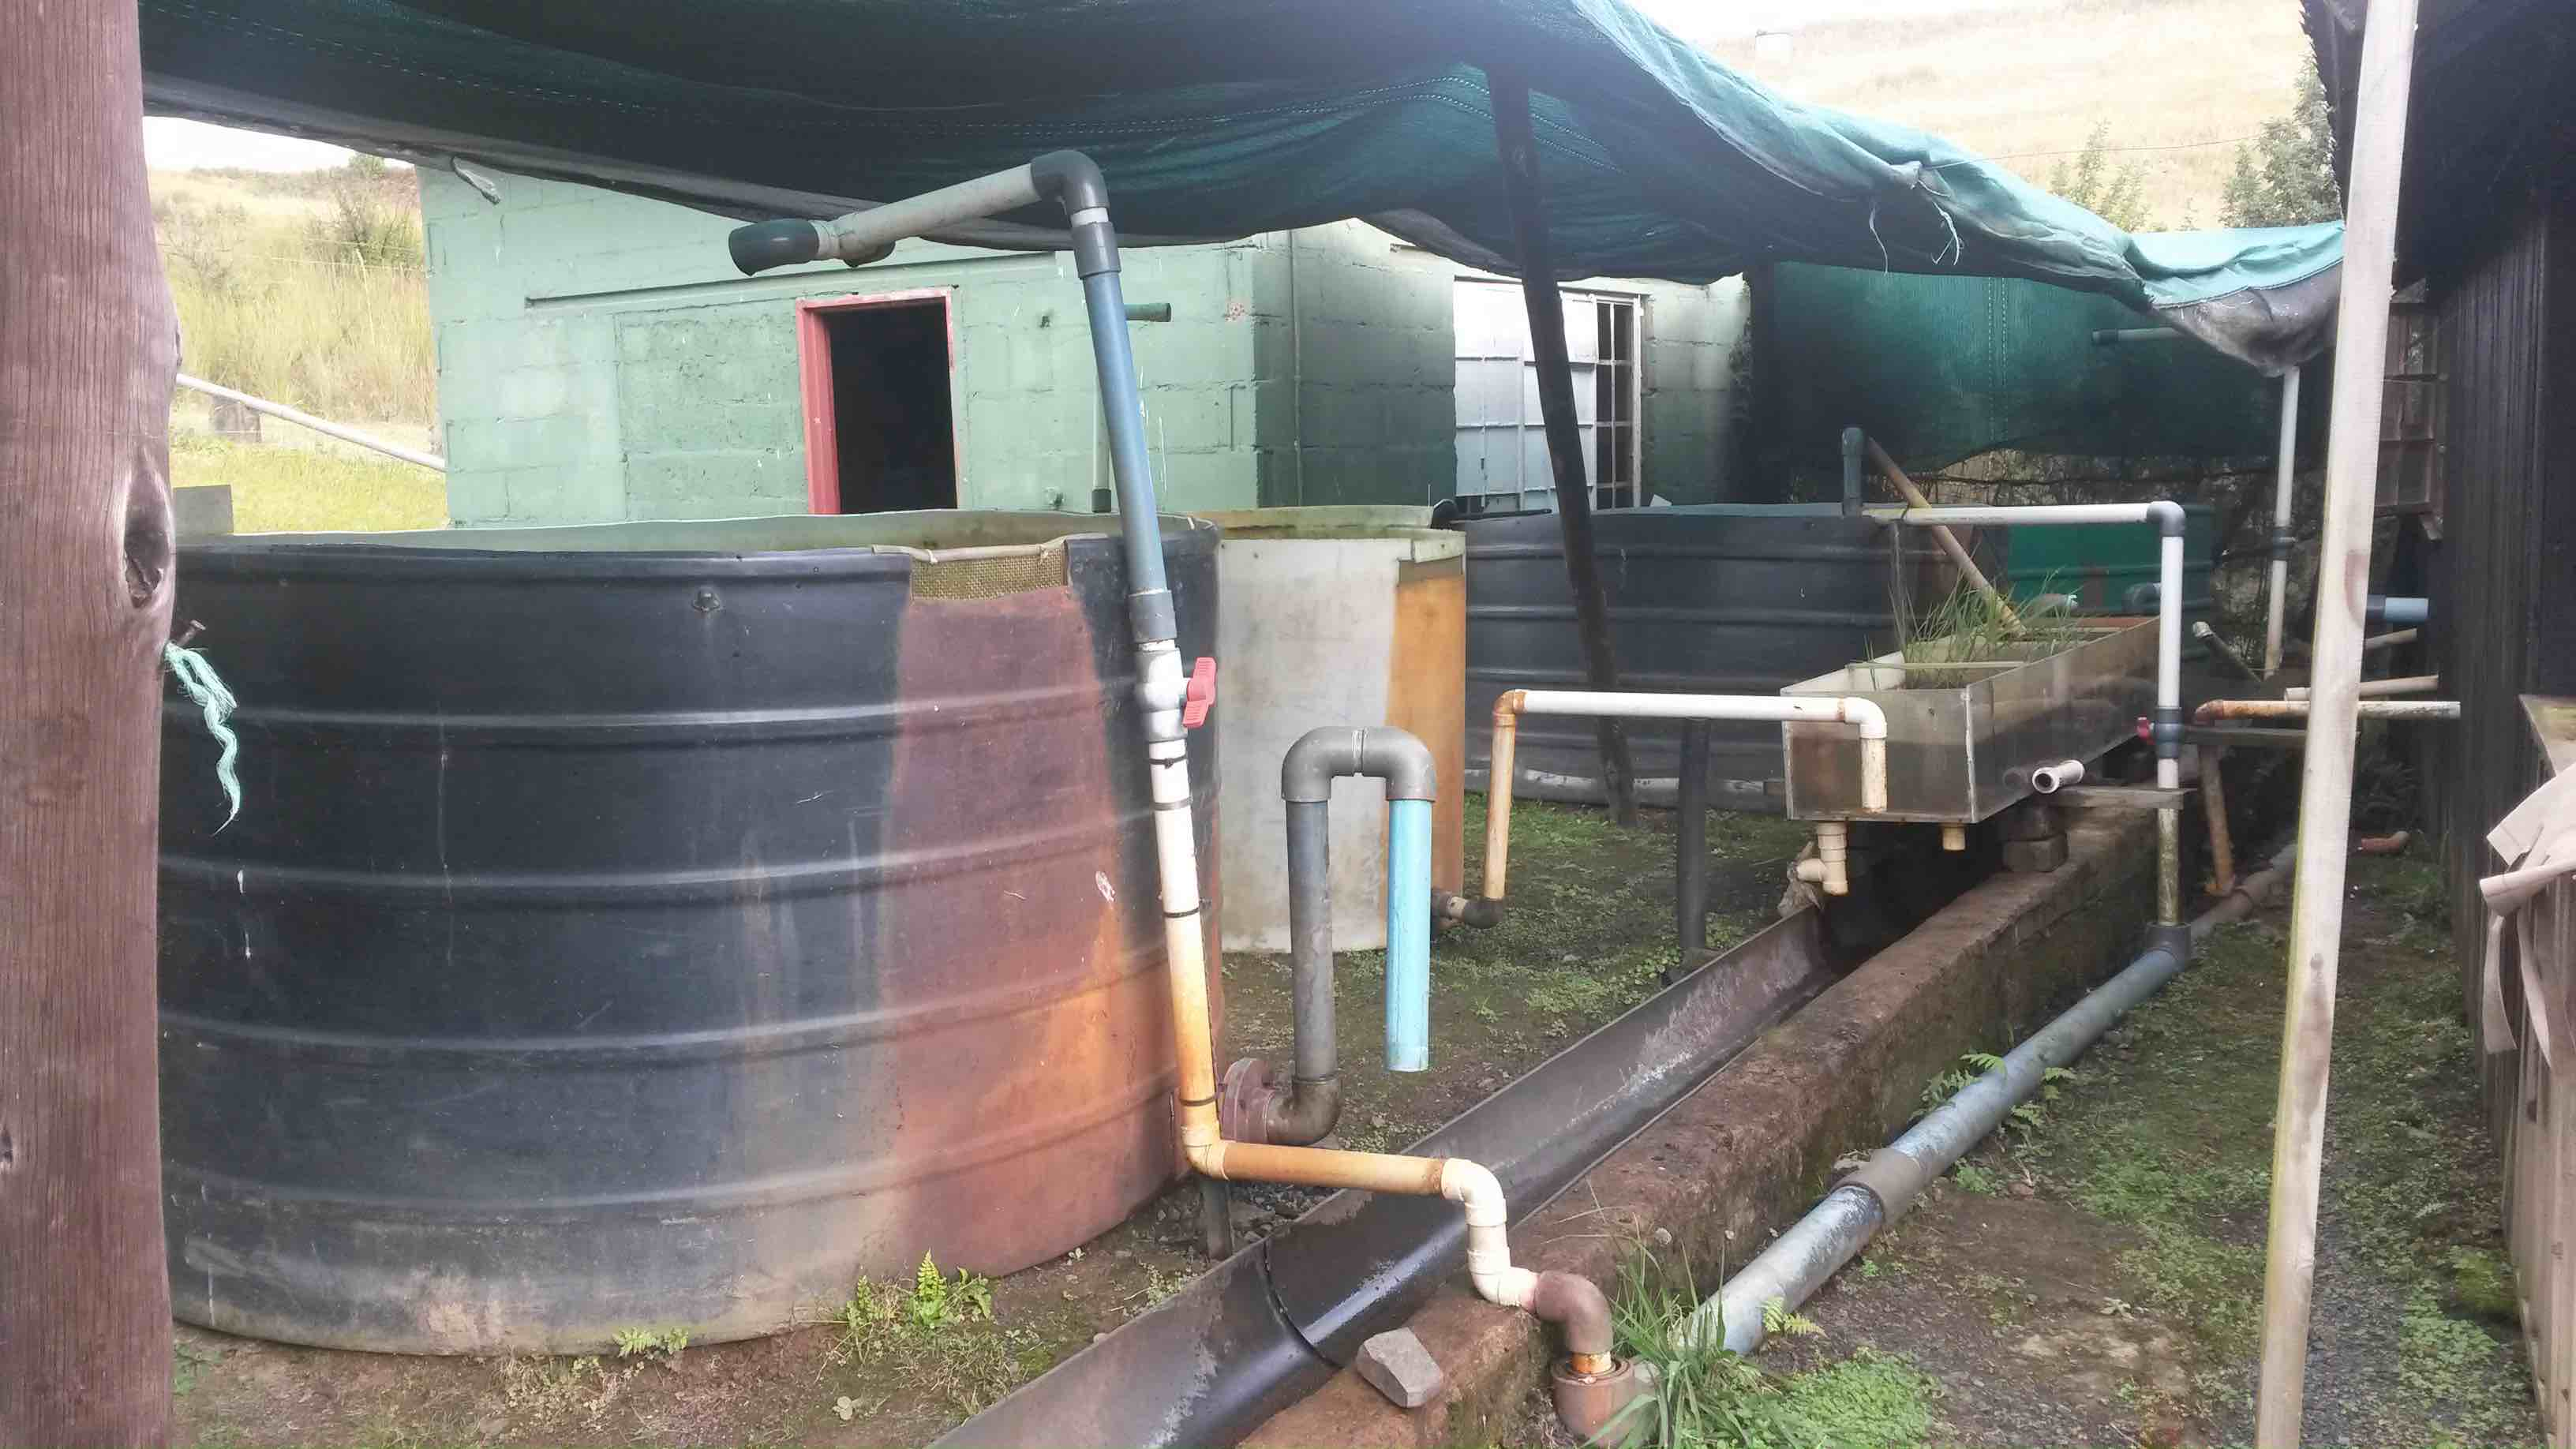
\includegraphics[scale = 0.1]{images/HatcheryTanks.jpg}
  \caption{Mbona fry tanks are plastic jojo type tanks used for rearing the fry till they are old enough to move to the tanks. The flow rate through the tank is controlled by an inlet valve and the depth of water in the tank is determined by the height of the overflow outlet pipe. }
   \label{fig:HatcheryTanks}
\end{figure}



\subsection{Growing Ponds}

\begin{figure}[H]
  \centering
   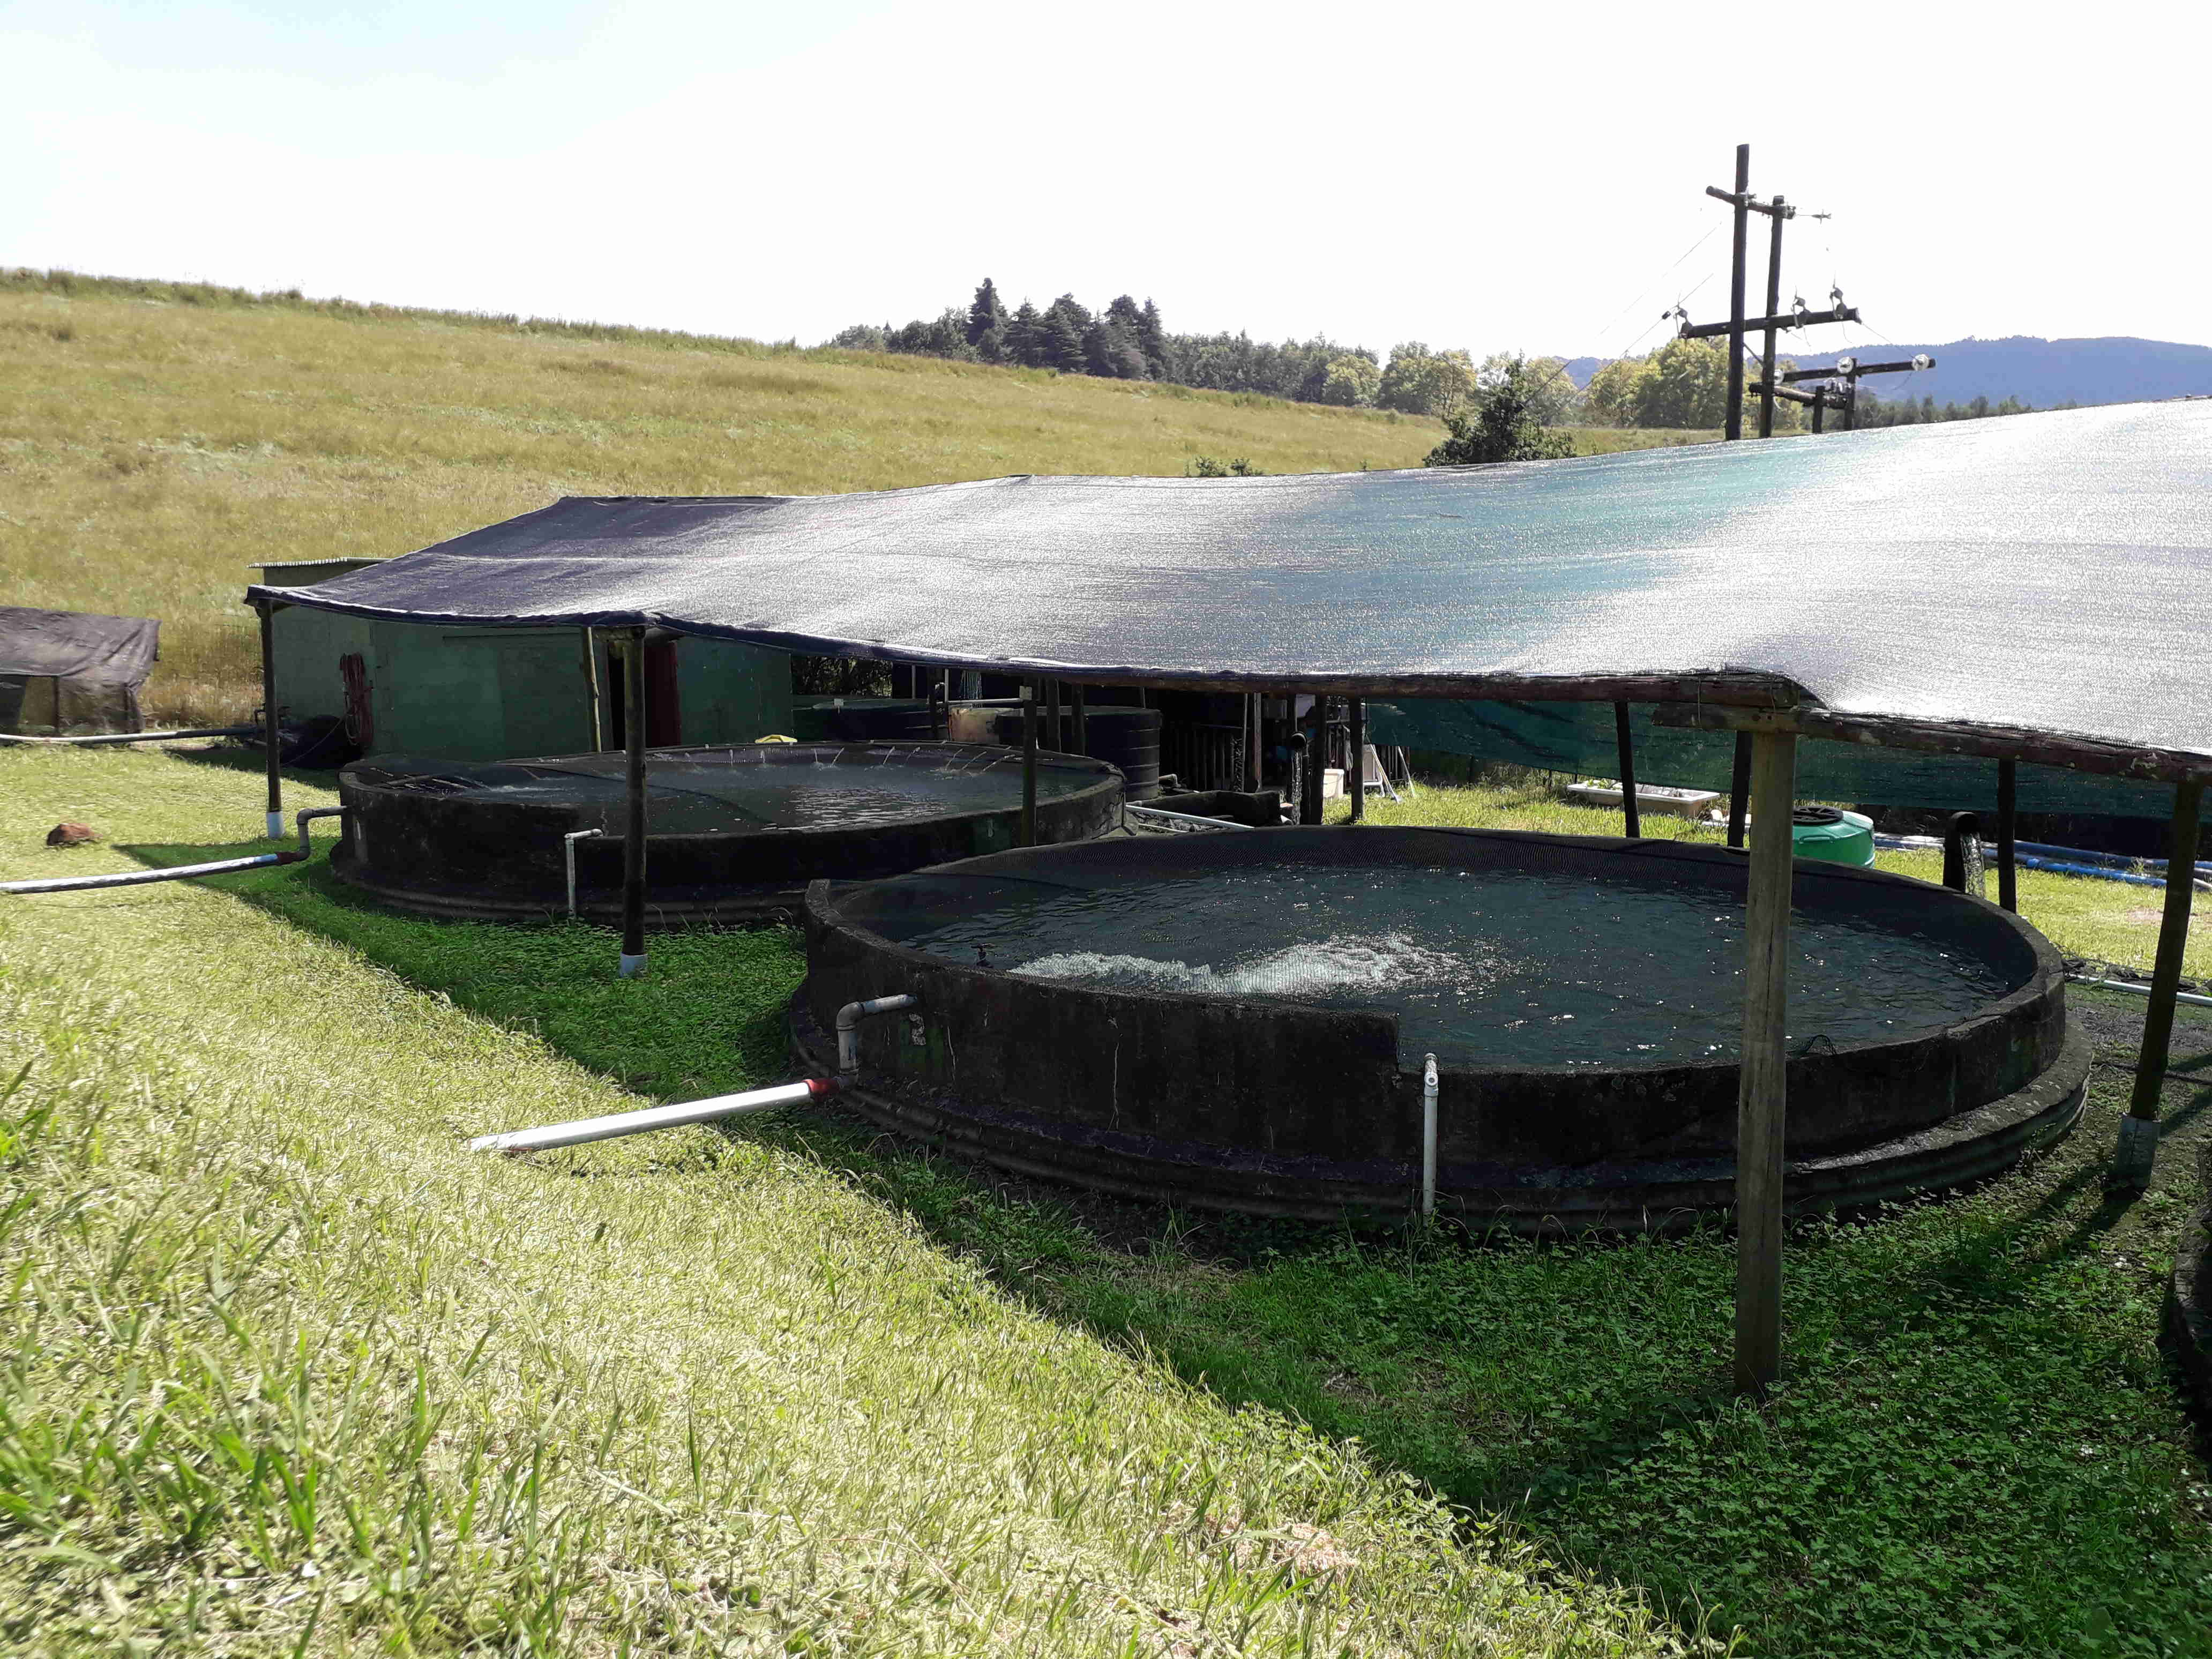
\includegraphics[scale = 0.1]{images/HatcheryPonds.jpg}
  \caption{Mbona growing ponds are of concrete construction and used for growing the fingerlings to sellable fish of length greater than 6 inches.  The flow rate through the pond is controlled by an inlet valve and the depth of water in the tank is determined by the height of the overflow outlet pipe. The ponds are covered with netting to prevent the fish from escaping. }
   \label{fig:HatcheryPonds}
\end{figure}



\subsection{Raceway}

\begin{figure}[H]
  \centering
   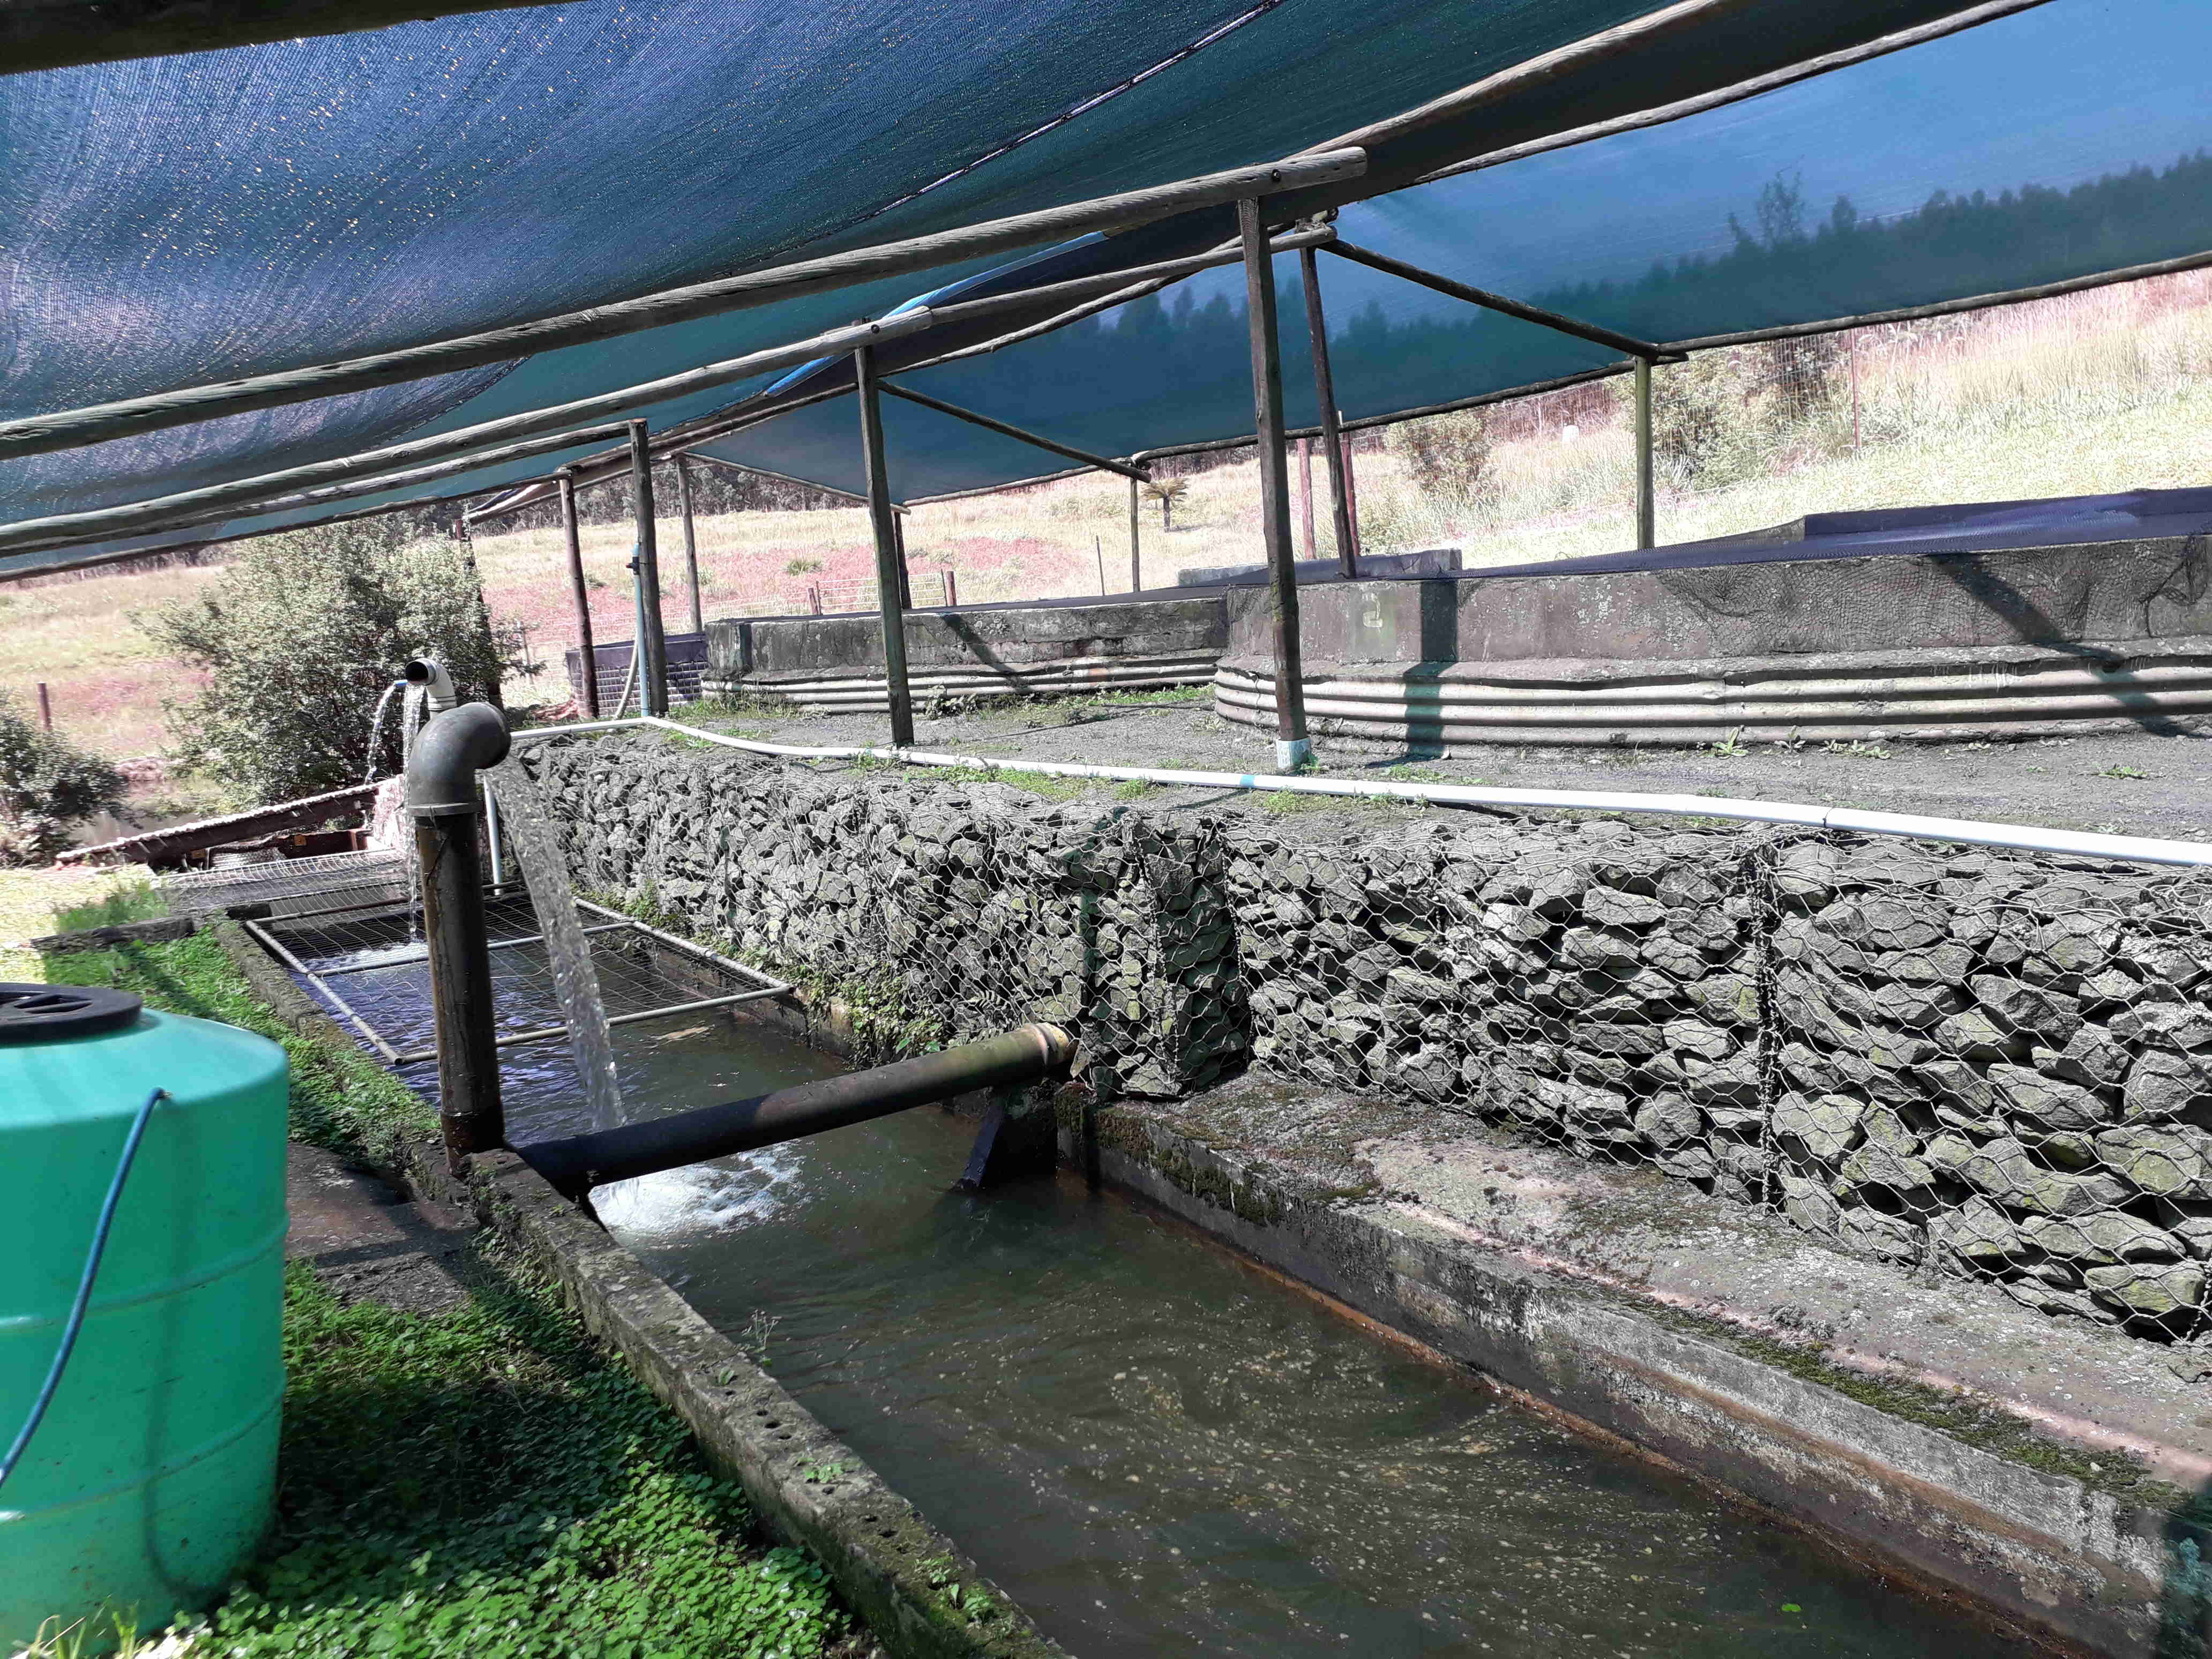
\includegraphics[scale = 0.1]{images/HatcheryRaceway.jpg}
  \caption{The Mbona raceway is used as an exit for the water after it has passed through the baths, tanks or ponds. It is also used to grow trophy and table fish for select customers.}
   \label{fig:HatcheryRaceway}
\end{figure}




\newpage
\section{Water Reticulation}

Water is siphoned from Lake Crystal and passed through an aeration tower before being piped to the baths, tanks, ponds and pools in the Mbona hatchery, see figure ~\ref{fig:HatcheriesWaterReticulation}. 

\begin{figure}[h]
  \centering
   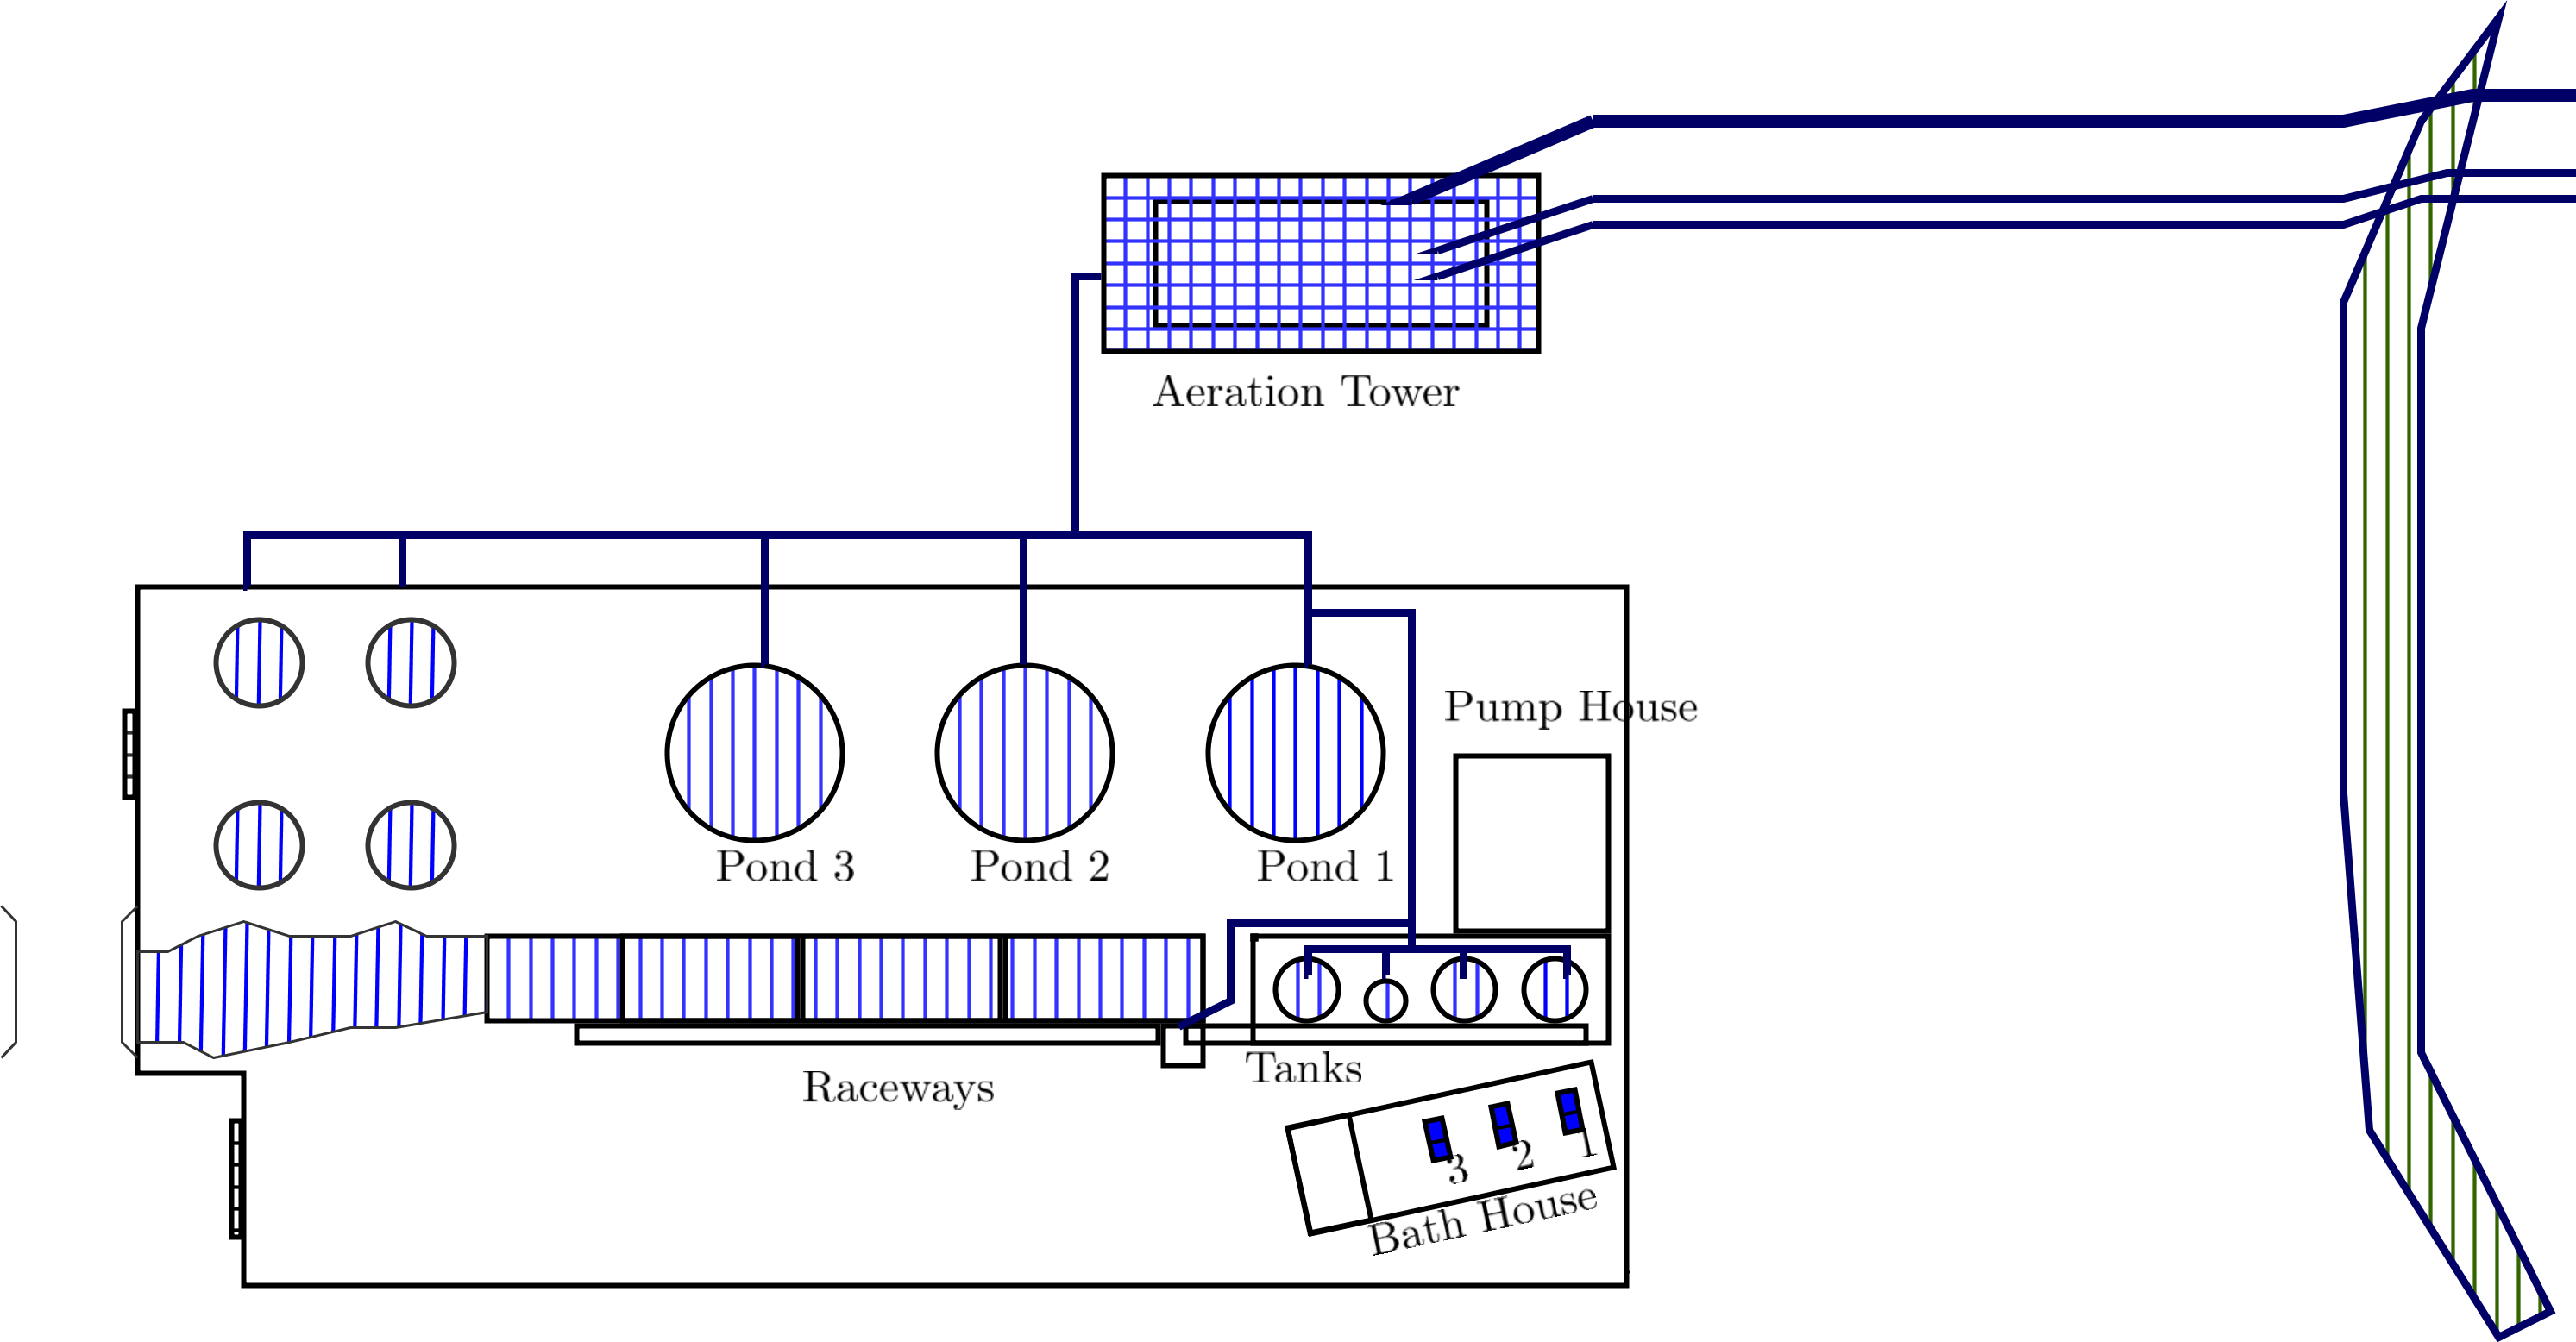
\includegraphics[scale = 0.15,angle=0,origin=c]{images/HatcheriesWaterReticulation.png}
  \caption{Mbona Hatcheries Water Reticulation System.}
   \label{fig:HatcheriesWaterReticulation}
\end{figure}

\subsection{Aeration Tower}

Aerated water is critical to the survival of live fish so The Mbona system used three different siphons to provide water to the aeration tower and on to the hatchery, see photgraph ~\ref{fig:HatcheryAerationTower}.

\begin{figure}[H]
  \centering
   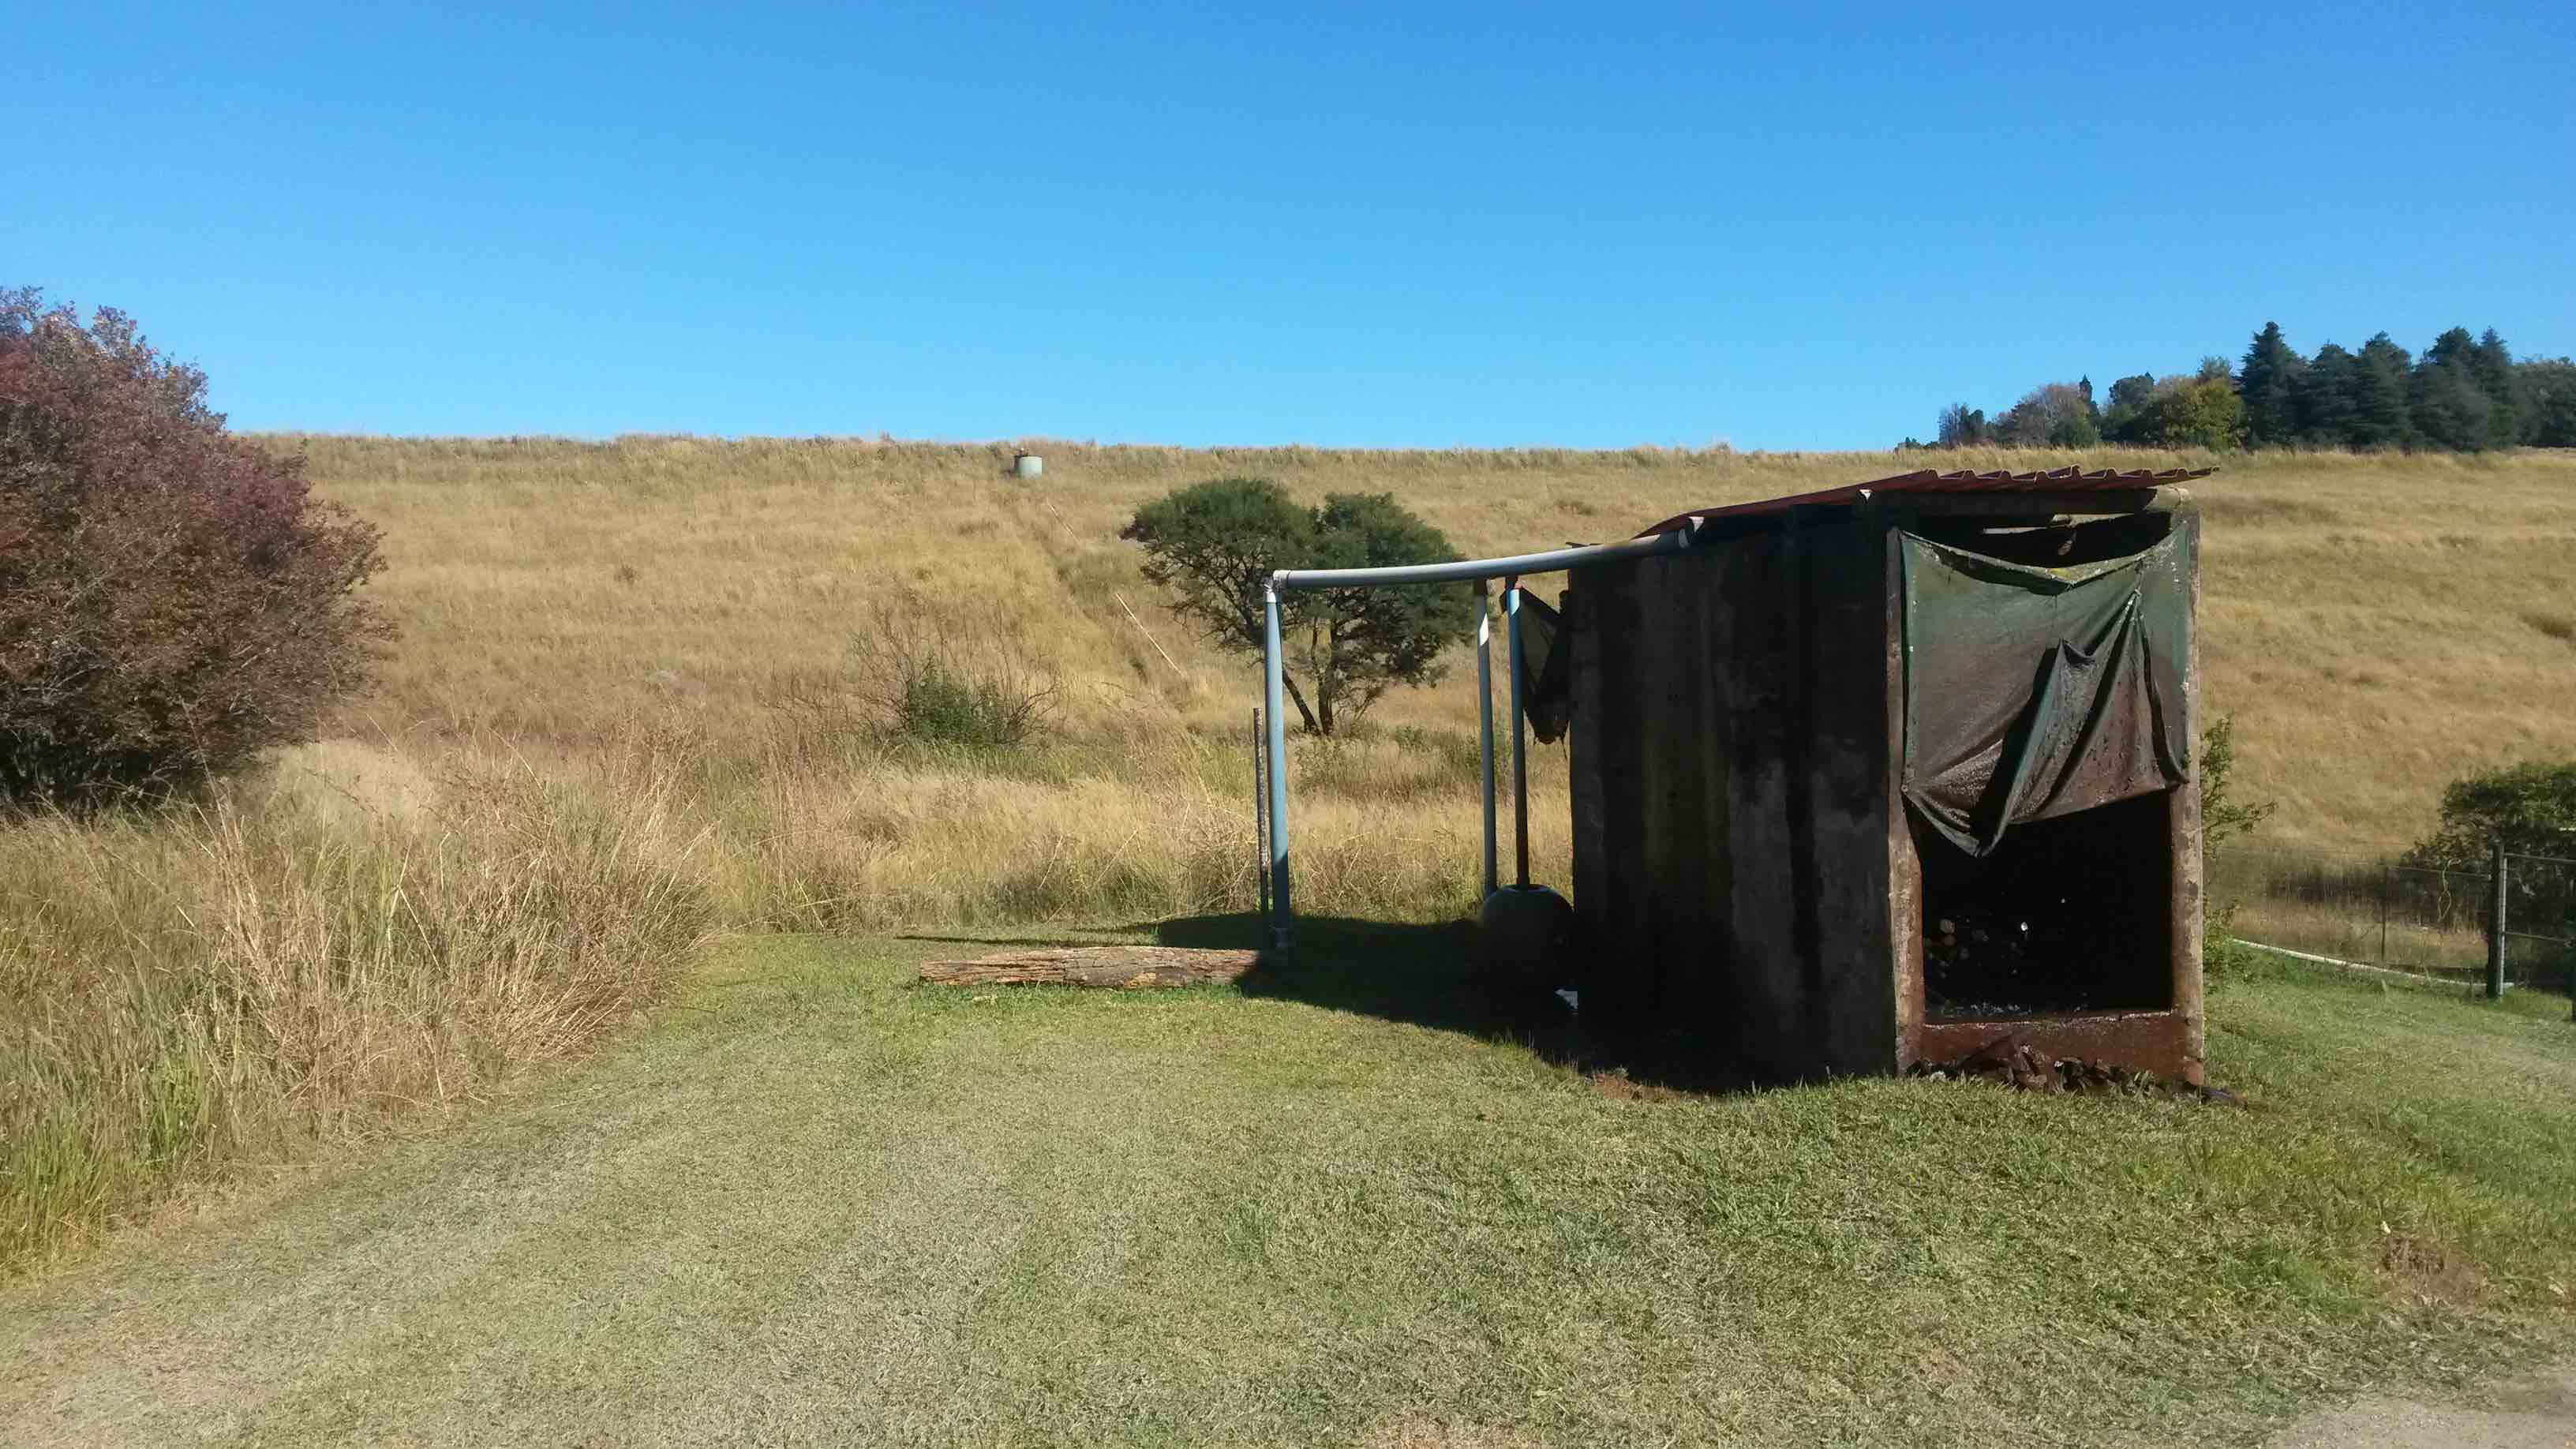
\includegraphics[scale = 0.1]{images/HatcheryAerationTower.jpg}
  \caption{The Mbona aeration tower is fed by {\bf three} siphons from Lake Crystal that must
  run continuously, see text for flow estimates.}
   \label{fig:HatcheryAerationTower}
\end{figure}


The flow of water from the three siphons can be computed using a formula outlined in the appendix of {\bf WaterPAK}, an Australian manual on best practices for the irrigation of cotton fields, see \cite{waterpak}.

The formula is based on Bernoulli's principle but adjusted for velocity loss due to friction between the water and the pipe. The flow rate for a siphon can be approximated by:

$$ Q = \frac{\pi D^2}{4} \sqrt{\frac{2 D H}{ 1.9 + 0.019 \frac{L}{D}} } $$

where

\begin{itemize}

\item[$Q$] is the flow rate in $m^3 s^{-1}$
\item[$D$] is the diameter of the siphon pipe in $m$
\item[$H$] is the height differential between the outlet and the lake surface in $m$.
\item[$L$] is the length of the siphon pipe in $m$.

\end{itemize}

Using this formula we compute daily discharge in litres expected from each of the 3 siphon pipes leading to the aeration tower. The results are presented in table ~\ref{tab:TablesSiphonVolume}.

\begin{table}[H]
  \centering
   
\includegraphics[scale = 0.8]{tables/TablesSiphonVolume.pdf}
   \caption{Siphon discharge in litres per day}
   \label{tab:TablesSiphonVolume}
\end{table}

These figures are supported by an experiment Pierre carried out when he use a bucket and stop watch to estimate the total consumption of the Hatchery with just the two smaller siphons feeding the aeration tower.
The results of this experiment are presented in table ~\ref{tab:TablesWaterConsumption}.

\begin{table}[H]
  \centering
   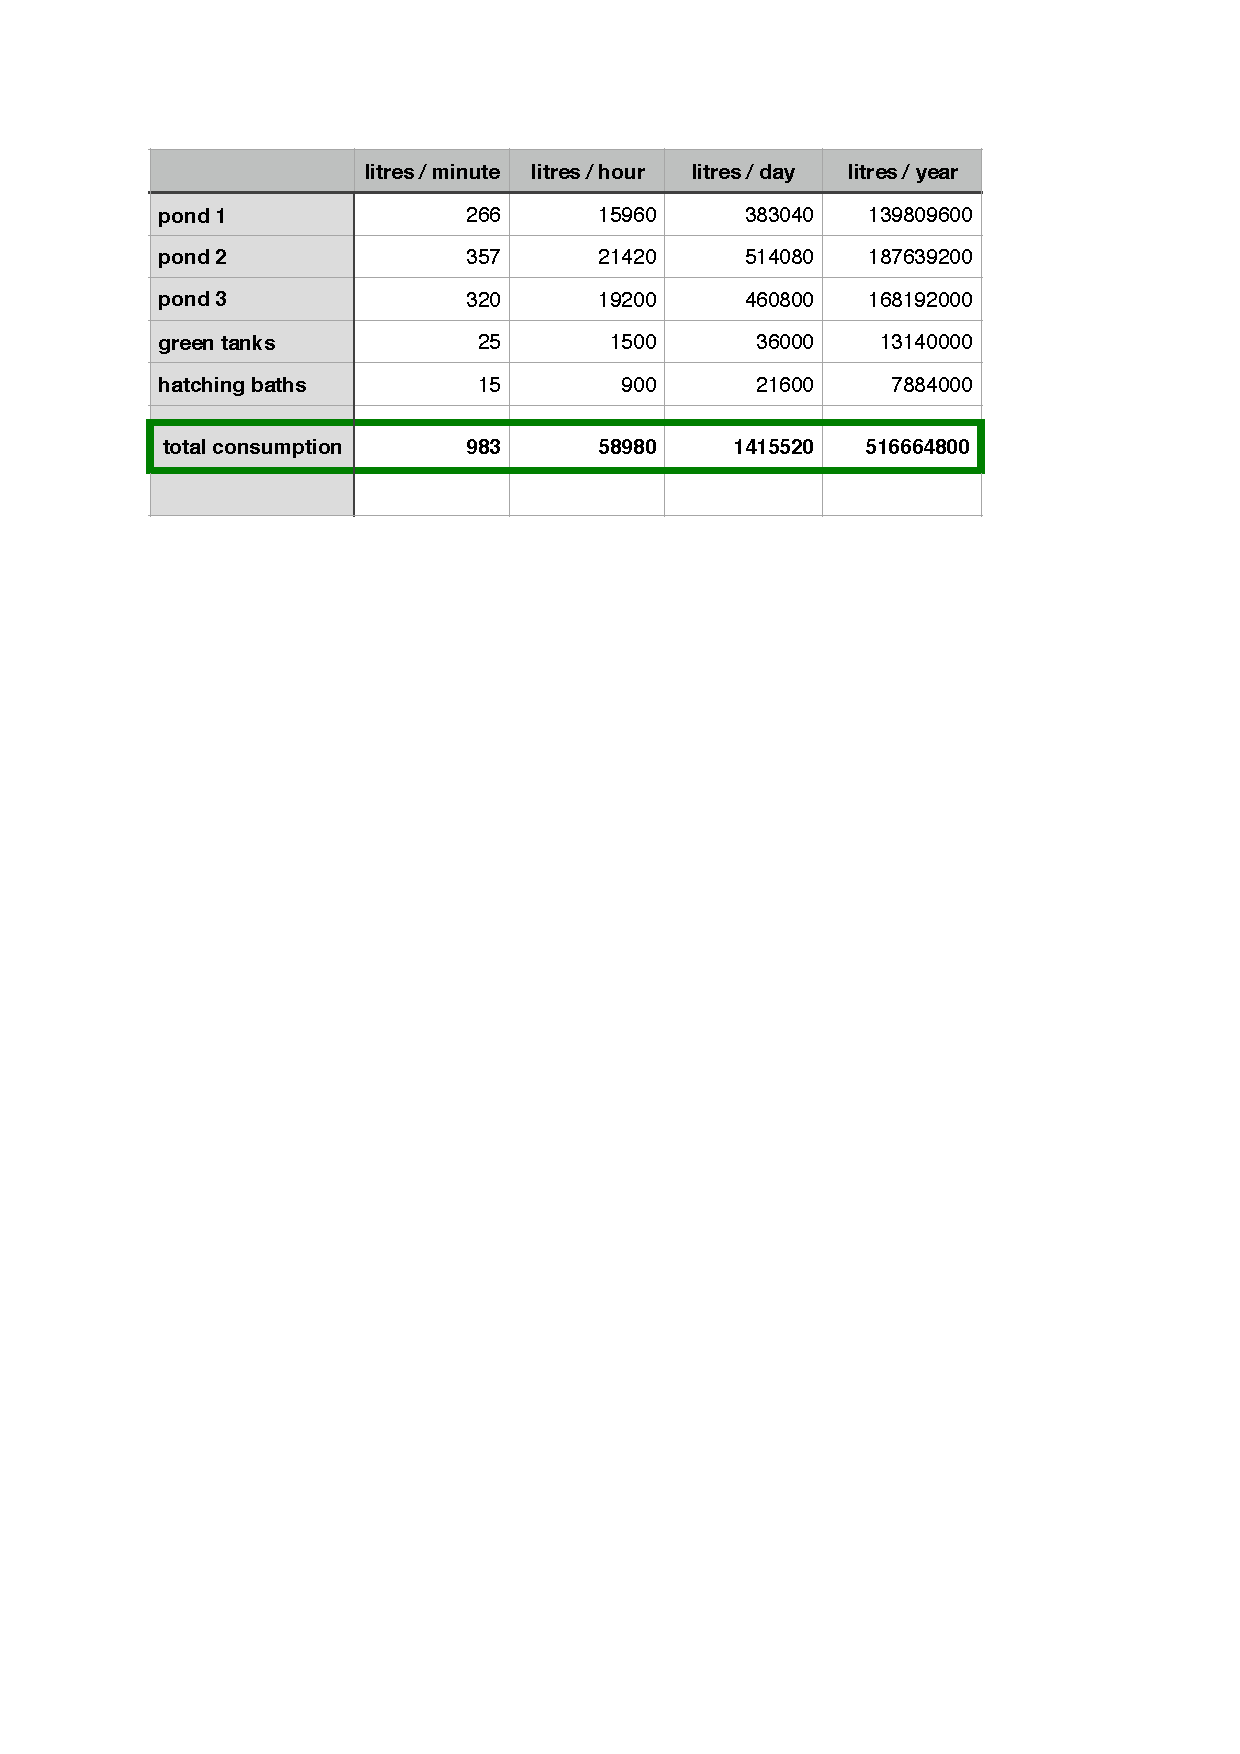
\includegraphics[scale = 0.8]{tables/TablesWaterConsumption.pdf}
   \caption{Water consumption in the Hatchery as measured with a bucket and stopwatch.}
   \label{tab:TablesWaterConsumption}
\end{table}







